In this section I am going to explore a new branch of the TSP resolution, in which the discovery of an optimal solution is no longer important. This development uses  matheuristic and heuristic to find a solution with a great approximation to the optimal one, even with instances including millions of nodes. Therefore, I am going to explore how big instances can be solved when classical methods such as MTZ and GG take too long. Moreover, I am going to cover different approach, namely matheuristic methods, heuristic and metaheuristic algoritms.


\section{Matheuristics}
"The objective of a heuristic is to produce a solution in a reasonable time frame that is good enough for solving the problem at hand. This solution may not be the best of all the solutions to this problem, or it may simply approximate the exact solution. But it is still valuable because finding it does not require a prohibitively long time"\cite{heuristic}.\\
The two techniques I am going to delve into are the hard-fixing and the soft-fixing.

\subsection{Hard-fixing}
\label{section:hard-fix}
The main purpose of this method is to try to reduce the search space by cutting down the complexity of the optimization. For achieving this goal, an initial feasible solution is needed - obtained by any approach described in this report.\\
The central thought of hard-fixing is to get an easier problem by setting some variables of the solution passed to the method - and so by having fewer variables to compute. The variables to be fixed are $x_{ij}$, $i, j\in V$. This task is done by settling the values to 1, so that the edge will be surely part of the solution. A valid method to choose which path is designated to be fixed is to link each edge to a probability $p$ between $0$ and $1$, then set randomly - with the probability picked - the value to 1.\\
Hereupon, the problem will presumably have $p*|E|$ variables fixed and thus the instance can be solved with a lower effort. Hopefully, this situation will bring to a better solution. Although the choice of using a probability is a good pick, any other method can be used to block the edges.

The performance of this technique is strictly related to the choice of the first feasible solution: if it is not good enough, this approach will get stuck on some non-optimal solution. A good fix for avoiding this is to lower down $p$ whenever the solution is not improved for a predetermined amount of time.

\begin{algorithm}
	\caption{Hard-fixing}\label{algo:hard-fix}
	\begin{algorithmic}[1]
		\Require $G=(V,E)$,$ c:E\rightarrow \Re^+$, $global\_timelimit$, $iteration\_timelimit$
		\Ensure $z\text{ hopefully good solution}$
		\State instance $\gets$ *initializing model (any of this report)*
		
		\State  $z$ $\gets$ \textsc{CPXmipopt} *with nodelimit 0*
		\State $p$ $\gets$ $0.9$
		\State $i$ $\gets$ $0$
		\While{$time\_elapsed<global\_time\_limit$}
			\If{$time\_remaining > iteration\_timelimit$}
				\State instance $\gets$ *set timelimit to $iteration\_timelimit$*
			\Else 
				\State instance $\gets$ *set timelimit to $time\_remaining$*
			\EndIf
			\State instance $\gets$ *hard-fixing with probability $p$*
			\State $z_{new}$ $\gets$ \textsc{CPXmipopt}
			
			\If{$cost(z_{new})<cost(z)$}
				\State $z$ $\gets$ $z_{new}$
				\State $i$ $\gets$ $0$
			\Else 
				\State $i$ $\gets$ $i+1$
			\EndIf
			
			\If{$i = 10$}
				\State $p$ $\gets$ $p - 0.1$
			\EndIf
			\State instance $\gets$ *remove hard-fixing*
		\EndWhile
		\State \Return $z$
	\end{algorithmic}
\end{algorithm}

In this algorithm, there are some variables not mentioned before: the global timelimit and the iteration timelimit. As aforementioned, the hard-fixing is a technique that aims to obtain a good solution in a short amount of time, so the parameters described above are necessary to establish - as the name suggests - the timespan in which the optimization is solved. global\_timelimit is the total time reserved to the solver, interation\_timelimit is the duration of each optimization in which the hard-fixing is applied.

The initial solution is provided by the solver, limited in the depth of its analysis. Then, algorithm \ref{algo:hard-fix} starts to iterate the main process until the global\_timelimit is reached. During this phase, the optimization is called several times, in each of which the instance is solved blocking some variables to $1$.

\subsection{Soft-fixing}
The technique that will be described is called Local Branching. Since it is a slight modification of the hard-fixing it is also called soft-fixing.\\
In section \ref{section:hard-fix} the value of the variables is fixed in a manual way using a probability system. In Local Branching, this operation is performed by adding a new constraint that forces the instance to block a predetermined number of variables, giving to the solver a degree of freedom on which variables to fix and which not.

The main idea of soft-fixing is the Hamming distance: "it measures the minimum number of substitutions required to change one string into the other"\cite{hamming-distance}. This description can be applied also to vectors. So given two vectors $x$ and $\tilde{x}$ in $\{0,1\}$, the Hamming distance is the number of different bits they have. It can be described in this way:

\begin{equation}
\label{eqn:hamming-dist}
H(x, \tilde{x}) = \sum_{j:\tilde{x}_j=1}(1-x_j)+\sum_{j:\tilde{x}_j=0}x_j
\end{equation}

Considering that the output solution of the solver is a vector in $\{0, 1\}$, it is possible to insert into the instance a new constraint that limits the hamming distance between the old solution and the new one.
The number of edges active in each solution is forced to be $n=|V|$ and therefore the Hamming distance is computed on the differences in the bits equal to 1. For this reason, it is possible to reduce \ref{eqn:hamming-dist} to:

\begin{equation}
\label{eqn:hamming-dist-2}
H(x, \tilde{x}) = \sum_{j:\tilde{x}_j=1}(1-x_j) =  n - \sum_{j:\tilde{x}_j=1}x_j
\end{equation}

The purpose of this method is to limit the diversity of two solutions. For doing so, it is possible to add a new variable $k$ that limits the Hamming distance. Through elementary math, this formulation is built as:

\begin{equation}
\label{eqn:hamming-dist-3}
H(x, \tilde{x}) \le k \Rightarrow n - \sum_{j:\tilde{x}_j=1}x_j \le k \Rightarrow \sum_{j:\tilde{x}_j=1}x_j \ge n - k
\end{equation}

The consequence of \ref{eqn:hamming-dist-3} is to narrow the next iteration of the optimization to a $k$-neighborhood of the previous one. As the method described in section \ref{section:hard-fix}, the value $k$ can vary if for the optimization doesn't improve the solution. 

\begin{algorithm}
	\caption{Soft-fixing}\label{algo:soft-fix}
	\begin{algorithmic}[1]
		\Require $G=(V,E)$,$ c:E\rightarrow \Re^+$, $global\_timelimit$, $iteration\_timelimit$
		\Ensure $z\text{ hopefully good solution}$
		\State instance $\gets$ *initializing model (any of this report)*
		
		\State  $z$ $\gets$ \textsc{CPXmipopt} *with nodelimit 0*
		\State $k$ $\gets$ $2$
		\State $i$ $\gets$ $0$
		\While{$time\_elapsed<global\_time\_limit$}
		\If{$time\_remaining > iteration\_timelimit$}
		\State instance $\gets$ *set timelimit to $iteration\_timelimit$*
		\Else 
		\State instance $\gets$ *set timelimit to $time\_remaining$*
		\EndIf
		\State instance $\gets$ *soft-fixing using a k-neighborhood*
		\State $z_{new}$ $\gets$ \textsc{CPXmipopt}
		
		\If{$cost(z_{new})<cost(z)$}
		\State $z$ $\gets$ $z_{new}$
		\State $i$ $\gets$ $0$
		\Else 
		\State $i$ $\gets$ $i+1$
		\EndIf
		
		\If{$i = 10$}
		\State $k$ $\gets$ $k + 1$
		\EndIf
		\State instance $\gets$ *remove soft-fixing*
		\EndWhile
		\State \Return $z$
	\end{algorithmic}
\end{algorithm}

The only changes between \ref{algo:hard-fix} and \ref{algo:soft-fix} are the variables used and the constraints added to the instance. In this implementation, $k$ is increased by $1$ every time the solution is not improved.

\section{Specialized heuristics}
In this section the concept of heuristic is explored in some of algorithms used to solve the TSP problem. In particular, a set of methods will be presented namely greedy algorithm, extra mileage, and 2-opt optimization.

\subsection{Greedy algorithm}
\label{sec:greedy}
This type of method is the easiest to understand and implement. This heuristic has its roots on the concept  of constructing the shortest path by connecting the nearest nodes.

This algorithm starts from an arbitrary node and chooses its following node by selecting the nearest one from the ones that are not already in the path. For this reason, it is also called Nearest Neighbor.

The main side effect is that the shortest path is easily missed since the last nodes - apart from special cases - are far from each othe and in this way the optimal solution is not selected. The algorithm is the following: 

\begin{algorithm}
	\caption{Greedy}\label{algo:greedy}
	\begin{algorithmic}[1]
		\Require $G=(V,E)$,$ c:E\rightarrow \Re^+$
		\Ensure $z\text{ hopefully good solution}$
		\State $best\_cost$ $\gets$ $+\infty$
		\State $z$ $\gets$ *empty*
		
		\For{$start\_node$ $\gets$1 $to$ n}
			\State $current\_node$ $\gets$ $start\_node$
			\While{*each node is visited*}
			\State $candidate\_node \gets$ $-1$
				\For{$i \gets 1$ $to$ n}
					\State *Finds the nearest node and marks it as visited*
					\State $candidate\_node \gets$ *nearest node*
				\EndFor
				\State *Saves $candidate\_node$ as next node*
				\State $current\_node$ $\gets$ $candidate\_node$
			\EndWhile
			\If{cost($z_{curr}$)$<best\_cost$}
				\State $best\_cost$ $\gets$ $cost(z_{curr})$
				\State $z$ $\gets$ $z_{curr}$
			\EndIf
		\EndFor
		\State \Return $z$
	\end{algorithmic}
\end{algorithm}

The classic implementation has a complexity of $O(n^2)$ since each node has to search the nearest node all over the graph. To obtain the best solution possible, in my implementation each node is tested as starting node. In particular, \ref{algo:greedy} has a complexity of $O(n^3)$ because of the aforementioned method to select the best starting node.\\
This complexity is quite low but it can be slower than expected with some instances over a great number of nodes.

\subsection{Extra mileage approach}
\label{sec:extra-mileage}
This approach is more complex than the previous one but in favor of a better solution. The main idea behind this algorithm is very simple and it sets up from an empty solution.

It starts by connecting the farthest nodes in the instance with a cycle, and this path will be the beginning of the solution. Then, the closest node among the active edges is selected and added to the solution by replacing it with two more edges that allow the new node to enter the solution. This process can be seen in figure \ref{fig:extra}, where it is performed with a five nodes.

\begin{figure}
	\centering
	\begin{subfigure}[b]{0.3\textwidth}
		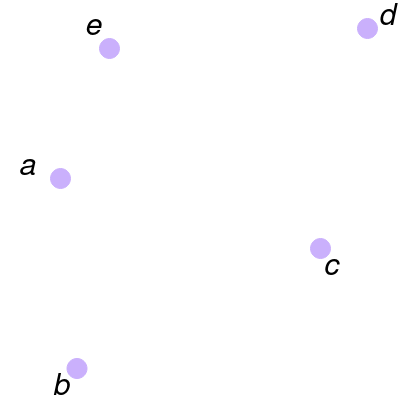
\includegraphics[width=\textwidth]{images/extra_1}
		\caption{No edges}
	\end{subfigure}
	\hfill
	\begin{subfigure}[b]{0.3\textwidth}
		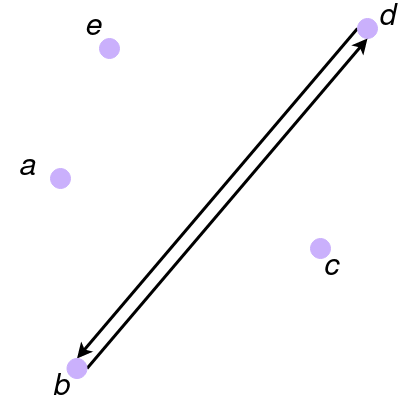
\includegraphics[width=\textwidth]{images/extra_2}
		\caption{First two edges added}
	\end{subfigure}
	\hfill
	\begin{subfigure}[b]{0.3\textwidth}
		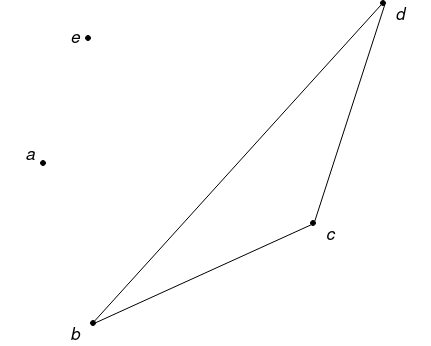
\includegraphics[width=\textwidth]{images/extra_3}
		\caption{One edge is substituted with other two connecting one more node}
	\end{subfigure}
	\bigskip
	\begin{subfigure}{0.3\textwidth}
		\centering
		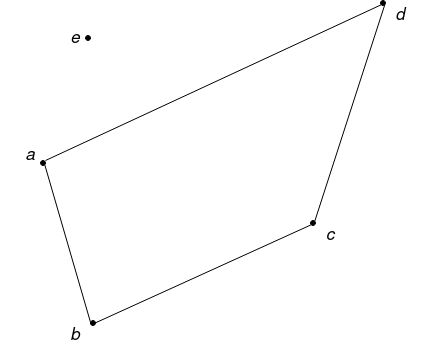
\includegraphics[width=\textwidth]{images/extra_4}
		\caption{Added one more node}
	\end{subfigure}
	\hfill
	\begin{subfigure}{0.3\textwidth}
		\centering
		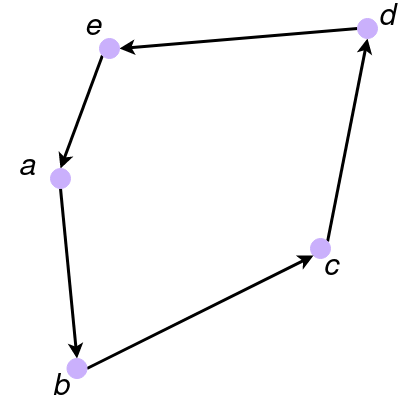
\includegraphics[width=\textwidth]{images/extra_5}
		\caption{All nodes are connected}
	\end{subfigure}
	\caption{In this image we can see the process done by extra-mileage to find the solution.}
	\label{fig:extra}
\end{figure}

For inserting the next node, the method used is the triangle inequality, which states that the sum of the lengths of any two sides must be greater than or equal to the length of the remaining side. In doing so with the replacing phase, some cost is added to the solution. Imagine taking into consideration three nodes $x$, $y$ and $z$, where $x$ and $y$ are already in the solution and $z$ wants to join them. The mathematical operation to apply is the following:

\begin{equation}
	\Delta(x, y, w) = c_{xw} + c_{yw} - c_{xy}
\end{equation}

This value will always be positive thanks to the aforementioned triangle inequality.

The algorithm used is the following:
\begin{algorithm}
	\caption{Extra mileage}\label{algo:extra-mileage}
	\begin{algorithmic}[1]
		\Require $G=(V,E)$,$ c:E\rightarrow \Re^+$
		\Ensure $z\text{ hopefully good solution}$
		\State $x, y$ $\gets$ *finds the farthest nodes*
		\State $z$ $\gets$ \textsc{Add($x, y$)}
		
		\While{$|z|<n$}
			\State $(x, y, w)$ $\gets$ argmin($\Delta(x, y, w):x, y \in z, w \not \in z$)
			\State $z$ $\gets$ \textsc{Add($w $)}
		\EndWhile
		\State \Return $z$
	\end{algorithmic}
\end{algorithm}

\subsection{2-opt refining}
This section analyzes a refining technique where the goal is to take an existing solution $x$ and to put it closer to the optimum one.\\
The $k$-opt refining consists on rearrange $k$ edges in order to obtain a new solution with a lower cost. In particular, this section describes the $2$-opt refining.

To handle this approach effectively, it is applied starting from a solution obtained with a heuristic approach - such as the ones described in section \ref{sec:greedy} and \ref{sec:extra-mileage}. The idea of this algorithm is to remove all the crossing edges and to insert new edges that will decrease the cost of the final solution.

Here too the triangle inequality is used to find the couple of edges that allow the best improvement. In this implementation, the operation is done across four nodes: $i$, $succ[i]$, $j$, and $succ[j]$. Since the tour is asymmetric, it has a direction: $succ[i]$ and $succ[j]$ are respectively the following nodes in the path of the nodes $i$ and $j$. 

\begin{equation}
	\label{eqn:2-opt}
	\Delta (i, j) = (c_{i, succ[i]} + c_{j, succ[j]}) - (c_{i, j} + c_{succ[i], succ[j]}) \quad i, j \in V; i\not=succ[j]; j\not=succ[i]
\end{equation}

In \ref{eqn:2-opt} it is described the correct way to compute the delta of the method. Greater the value, better the improving.

\begin{figure}[h]
	\centering
	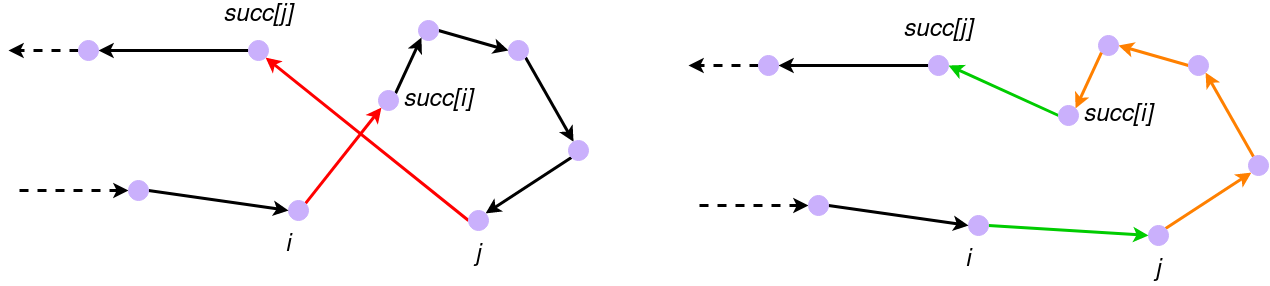
\includegraphics[width=0.9\textwidth]{images/2_opt_new.png}
	\caption{The image represent the replacement of two edges during the $2$-opt refining.}
	\label{fig:2-opt}
\end{figure}

In figure \ref{fig:2-opt} it is possible to look at the replacement of two arcs. It is important to notice that the path from $i$ to $succ[i]$ changes direction after the substitution of the old edges. This is done for maintaining the solution integrity. In particular, this optimization is performed until no more positive $\Delta(i, j)$ are found. If they are not found, the solution is no more improvable by the 2-opt algorithm.

\begin{algorithm}
	\caption{$2$-opt refining}\label{algo:2-opt}
	\begin{algorithmic}[1]
		\Require $G=(V,E)$,$ c:E\rightarrow \Re^+$
		\Ensure $z\text{ hopefully good solution}$
		\State $z$ $\gets$ *find feasible solution with an algorithm*
		\State flag $\gets$ $false$
		
		\While{$flag==false$}
			\State flag $\gets$ $true$
			\State $(i, j)$ $\gets$ argmax($\Delta(i, j):i, j\in V)$
			\If{$\Delta(i, j)>0$}
				\State flag $\gets$ $false$
				\State $z$ $\gets$ *edge replacement*
			\EndIf
		\EndWhile
		\State \Return $z$
	\end{algorithmic}
\end{algorithm}

\begin{figure}
	\centering
	
	\begin{subfigure}[b]{0.45\textwidth}
		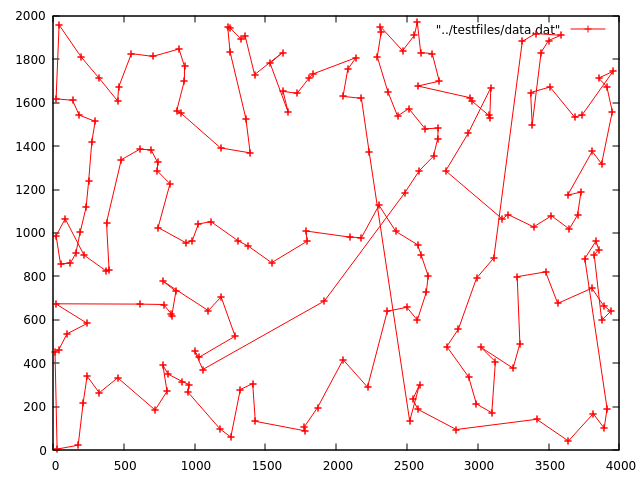
\includegraphics[width=\textwidth]{images/kroA_greedy.png}
	\end{subfigure}
	\hfill
	\begin{subfigure}[b]{0.45\textwidth}
		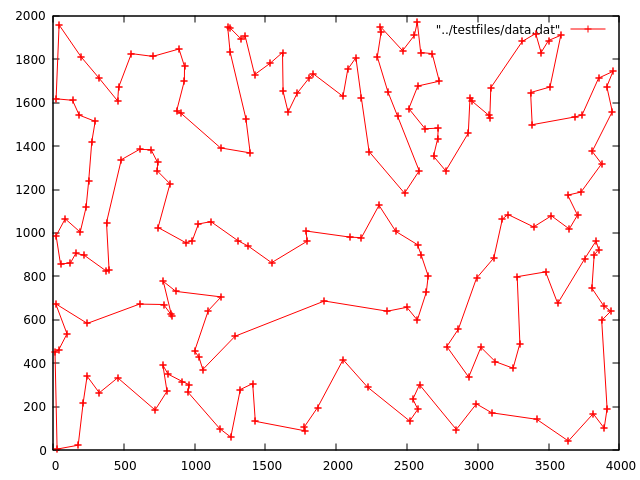
\includegraphics[width=\textwidth]{images/2_opt.png}
	\end{subfigure}
	\caption{The improvement obtained applying to a greedy algorithm (left) the 2-opt refining approach (right).}
\end{figure}

\section{Metaheuristics}
\label{chapter:metaheuristics}
While the heuristic approach seen before was strictly specific to the TSP problem, the concept of metaheuristic is quite different. Their procedure is problem-independent and does not take advantage of any specificity of the problem. Generally, these techniques are not greedy and can accept a temporary deterioration of the solution in order to have a bigger search space in which to find a better solution.

In this section, some of them will be used such as the variable neighborhood search and the tabu search.

\subsection{Variable Neighborhood Search}
\label{sec:VNS}
The variable neighborhood search (VNS) is the first metaheuristic approach presented. Its main purpose is to try to escape from a local optimal of the solution aiming to find the optimal solution of the problem. 

The instance of the problem can be seen as a function with its local minima, local maxima, and so on. During the utilization of some heuristic techniques, it is possible that the process remains stuck in a sub-optimal area. The way in which it tries to escape from this region is done by changing the \textit{neighborhood} of the solution: some data are modified and then a new minimum is searched.

In this report, the adjustment of the neighborhood is performed by a perturbation phase in which is applied a $k$-opt kick. This change is performed by selecting randomly a $k$ set of edges and then replacing them with others in order to obtain a poor solution. In particular, the procedure done is the following: a $2$-opt refining is applied to a reference solution, once the minimum is reached a kick is given to the solution to worsening the solution. Then the $2$-opt refining approach is used again to find a new minimum. In my implementation are implemented three perturbations: 3, 5, and 7. An example of implementation can be seen in Algorithm \ref{algo:vns}.

\begin{algorithm}
	\caption{VNS}\label{algo:vns}
	\begin{algorithmic}[1]
		\Require $G=(V,E)$,$ c:E\rightarrow \Re^+, k, global\_timelimit$
		\Ensure $z\text{ hopefully good solution}$
		\State $z_{curr}$ $\gets$ $z$ $\gets$ *built solution using an heuristc*
		\State $best\_cost$ $\gets$ cost($z$)
		\State cycles $\gets$ $0$
		\While{$time\_elapsed<global\_timelimit$}
			\State $z_{curr}$ $\gets$ \textsc{2-opt($z_{curr}$)}
			\If{cost($z_{curr}$) $< best\_cost$}
				\State z $\gets$ $z_{curr}$
				\State $best\_cost$ $\gets$ cost($z_{curr}$)
			\EndIf
		\State *Bigger the value of cycles bigger the kick*
		\State $z_{curr}$ $\gets$ \textsc{k-kick($cycles$)}
		\State cycles $\gets$ cycles$+1$
		\EndWhile
		\State \Return $z$
	\end{algorithmic}
\end{algorithm}


\subsection{Tabu search}
\label{sec:tabu-search}
The tabu search is the second metaheuristic presented in this report. It is a method to improve the local search and avoid falling back in a previous local minimum. To do that the concept of tabu is introduced: a set of banned solutions prevents the algorithm to return an already visited result.

In this implementation of the tabu search the refining phase is performed by a 2-opt move as it happened in section \ref{sec:VNS}, then the method to escape from this minimum is to perform a kick like as the previous section. The main difference is that during the VNS is possible to fall again and again in the previous solution, using the tabu search is not possible. 

The worsening move is performed by swapping two non-consecutive edges, then they are declared as tabu: they cannot be swapped for a while. This process precludes the possibility of falling into a cycle of deterioration-recover, where to final solution is always the same. This algorithm will continuously worsen the solution until a non-tabu move is performed.

The way in which this method is implemented is the following: each time a worsening action is performed the nodes selected are declared as tabu and the edges connected with them cannot be changed by any improving moves. If each time this action has been performed the list of tabu nodes becomes so large that no more moves are allowed. To avoid this case it is introduced a new variable called $tenure$, its main idea is to limit how many times a tabu is valid.

To do that we declare a node tabu (for example $i$) by inserting into an array the iteration number $h$, so $tabu\_nodes[i] = h$. This constraint will last for a $tenure$ number of times, following this rule:

\begin{equation}
	iteration\_number - tabu[i] \le tenure
\end{equation}

A good choice of $tenure$ is crucial to allow the algorithm to perform adequately. The best decision is to make it variable regarding the number of iterations already completed. In algorithm \ref{algo:tabu-search} can be seen the proceeding of this method.

\begin{algorithm}
	\caption{Tabu search}\label{algo:tabu-search}
	\begin{algorithmic}[1]
		\Require $G=(V,E)$,$ c:E\rightarrow \Re^+, k, global\_timelimit$
		\Ensure $z\text{ hopefully good solution}$
		\State $z_{curr}$ $\gets$ $z$ $\gets$ *built solution using an heuristc*
		\State $best\_cost$ $\gets$ cost($z$)
		\State $iteration\_counter \gets 1$
		\While{$time\_elapsed<global\_timelimit$}
			\State *Performs a 2-opt refining applying the constaraint described in section \ref{sec:tabu-search}. The iteration counter is increased each time a move is performed. If no moves are allowed this method does nothing*
			\State $z_{new}$ $\gets$ \textsc{tabu-2-opt($z_{curr}, tabu, tenure, iteration\_counter$)}
			\If{cost($z_{curr}$) $< best\_cost$}
				\State z $\gets$ $z_{curr}$
				\State $best\_cost$ $\gets$ cost($z_{curr}$)
			\EndIf
			\State $first\_node \gets RANDOM(|V|)$
			\State $second\_node \gets RANDOM(|V|)$
			\State $tabu[first\_node] \gets iteration\_counter$
			\State $tabu[second\_node] \gets iteration\_counter$
			\State $z_{curr} \gets $ \textsc{2-kick($first\_node, second\_node$)}
			\State $iteration\_counter \gets iteration\_counter+1$
		\EndWhile
		\State \Return $z$
	\end{algorithmic}
\end{algorithm}

\subsection{Genetic algorithms}